\documentclass[spanish]{beamer}
\usepackage[ansinew]{inputenc} % Acepta caracteres en castellano
\usepackage[spanish]{babel}    % silabea palabras castellanas
\usepackage{amsmath}
\usepackage{mathtools,cancel} % cancela con una flecha \cancelto{0}{XXXX}
\renewcommand{\CancelColor}{\color{red}} %change cancel color to red
\usepackage{amsfonts}
\usepackage{amssymb}
\usepackage{dsfont}
\usepackage{graphicx}
\usepackage{geometry}
\usetheme{Madrid}
\usecolortheme{beaver}
\usepackage{textpos}
% Logo  en el comienzo 
\addtobeamertemplate{frametitle}{}{%
\begin{textblock*}{100mm}(.85\textwidth,-1cm)
{\includegraphics[height=0.4in, keepaspectratio=true]{/Users/luisnunez/Dropbox/MisDocumentos/UIS/UISImagenInstitucional/UISLOGO.png}}
\end{textblock*}}

\begin{document}

\title{\textbf{Cuerpo R�gido: Energ�a cin�tica} }
\author[L.A. N��ez]{\textbf{Luis A. N��ez}}  
\institute[UIS]{\textit{Escuela de F�sica, Facultad de Ciencias, } \\
\textit{Universidad Industrial de Santander, Santander, Colombia } \\
{\includegraphics[height=0.4in, keepaspectratio=true]{/Users/luisnunez/Dropbox/MisDocumentos/UIS/UISImagenInstitucional/UISLOGO.png}}
}
\date{\today}
\maketitle


\begin{frame}
\frametitle{Agenda}
  \tableofcontents
\end{frame}


%%%%% Diapo 1
\section{La energ�a cin�tica}
\frame{
\frametitle{La energ�a cin�tica}
\begin{itemize}  
	\item<1-> La energ�a potencial de interacci�n entre las part�culas de un cuerpo r�gido es constante.  
	\item<2-> Entonces toda la energ�a potencial del s�lido es la energ�a potencial del centro de masa.
	\item<3-> La energ�a cin�tica de un cuerpo r�gido con velocidad angular $\boldsymbol{\Omega}$, es
	$T=\frac{1}{2} \sum_j^{\text {cuerpo }} m_j v_j^2, \quad j=1,2, \ldots$, donde $\mathbf{v}_j=\mathbf{v}_{\mathrm{cm}}+\boldsymbol{\Omega} \times \mathbf{r}_j,$
	\item<4->  Como la velocidad angular $\boldsymbol{\Omega}$ es la misma para todas las part�culas del cuerpo, tenemos
	$T  =\frac{1}{2} \sum_j m_j\left(\mathbf{v}_{\mathrm{cm}}+\boldsymbol{\Omega} \times \mathbf{r}_j\right)^2$, es decir \\ $T =\frac{1}{2} \sum_j m_j v_{\mathrm{cm}}^2+\sum_j m_j \mathbf{v}_{\mathrm{cm}} \cdot\left(\boldsymbol{\Omega} \times \mathbf{r}_j\right)+\frac{1}{2} \sum_j m_j\left(\boldsymbol{\Omega} \times \mathbf{r}_j\right)^2$
	\item<5-> El primer t�rmino es $\frac{1}{2} \sum_j m_j v_{\mathrm{cm}}^2=\frac{1}{2}\left(\sum_j m_j\right) v_{\mathrm{cm}}^2=\frac{1}{2} M v_{\mathrm{cm}}^2$.
	\item<6-> El segundo t�rmino se simplifica usando $\mathbf{a} \cdot(\mathbf{b} \times \mathbf{c})=\mathbf{b} \cdot(\mathbf{c} \times \mathbf{a})=\mathbf{c} \cdot(\mathbf{a} \times \mathbf{b})$.  Entonces
	$\sum_j m_j \mathbf{v}_{\mathrm{cm}} \cdot\left(\boldsymbol{\Omega} \times \mathbf{r}_j\right)  =\sum_j m_j \mathbf{r}_j \cdot\left(\mathbf{v}_{\mathrm{cm}} \times \boldsymbol{\Omega}\right) =$ $=\left(\mathbf{v}_{\mathrm{cm}} \times \boldsymbol{\Omega}\right) \cdot \cancelto{0}{\left(\sum_j m_j \mathbf{r}_j\right)}=0$, ya que  $\mathbf{R}_{\mathrm{cm}}=\frac{\sum_j m_j \mathbf{r}_j}{M}=0$

\end{itemize}
}
%%%%% Diapo 2
\section{El Tensor de Inercia}
\frame{
\frametitle{El Tensor de Inercia}
\begin{itemize}  
	\item<1-> El tercer t�rmino se eval�a usando $(\mathbf{a} \times \mathbf{b}) \cdot(\mathbf{c} \times \mathbf{d})=(\mathbf{a} \cdot \mathbf{c})(\mathbf{b} \cdot \mathbf{d})-(\mathbf{a} \cdot \mathbf{d})(\mathbf{b} \cdot \mathbf{c})$, por lo tanto
	$\left(\boldsymbol{\Omega} \times \mathbf{r}_j\right)^2=\left(\boldsymbol{\Omega} \times \mathbf{r}_j\right) \cdot\left(\boldsymbol{\Omega} \times \mathbf{r}_j\right)=\Omega^2 r_j^2-\left(\boldsymbol{\Omega} \cdot \mathbf{r}_j\right)^2$
	\item<2-> Entonces $T =\frac{1}{2} M v_{\mathrm{cm}}^2+\frac{1}{2} \sum_j m_j\left[\Omega^2 r_j^2-\left(\boldsymbol{\Omega} \cdot \mathbf{r}_j\right)^2\right]  =T_{\mathrm{cm}}+T_{\mathrm{rot}}$
	\item<3-> Adem�s, $\left(\boldsymbol{\Omega} \cdot \mathbf{r}_j\right)^2  =\left(\sum_i \Omega_i x_{i \, j}\right)\left(\sum_k \Omega_k x_{i \, j}\right)=\sum_{i, k} \Omega_i \Omega_k x_{i \, j} x_{i \, j},$, $\Omega_i  =\sum_k \Omega_k \delta_{i k}, \quad \Rightarrow \Omega^2  =\sum_i \Omega_i^2=\sum_i \Omega_i \sum_k \Omega_k \delta_{i k}=\sum_{i, k} \Omega_i \Omega_k \delta_{i k}$
	\item<4-> La energ�a cin�tica ser� $T_{\text {rot }}  =\frac{1}{2} \sum_j^{\text {cuerpo }} m_j \sum_{i, k}\left(\Omega_i \Omega_k r_j^2 \delta_{i k}-\Omega_i \Omega_k x_i x_k\right) $, o mejor 
	$T =\frac{1}{2} \sum_{i, k} \Omega_i \Omega_k \sum_j m_j\left(r_j^2 \delta_{i k}-x_i x_k\right) \equiv \frac{1}{2} \sum_{i, k} I_{i k} \Omega_i \Omega_k$
	\item<5-> Donde $I_{i j} =\left(\begin{array}{ccc}\sum_j m_j\left(x_2^2+x_3^2\right) & -\sum_j m_j x_1 x_2 & -\sum_j m_j x_1 x_3 \\ -\sum_j m_j x_2 x_1 & \sum_j m_j\left(x_1^2+x_3^2\right) & -\sum_j m_j x_2 x_3 \\ -\sum_j m_j x_3 x_1 & -\sum_j m_j x_3 x_2 & \sum_j m_j\left(x_1^2+x_2^2\right)\end{array}\right)$
\end{itemize}
}
%%%%% Diapo 2
\section{Elipsoide en rotaci�n}
\frame{
\frametitle{Elipsoide en rotaci�n}
\begin{itemize}  
	\item<1-> Energ�a cin�tica de un elipsoide ( $I_{11} \neq I_{22} \neq I_{33}$ ) que rota sobre eje $A B$ con velocidad angular $\omega$, y sobre eje $C D$ con velocidad angular $\nu$,
	\begin{figure}[t]
		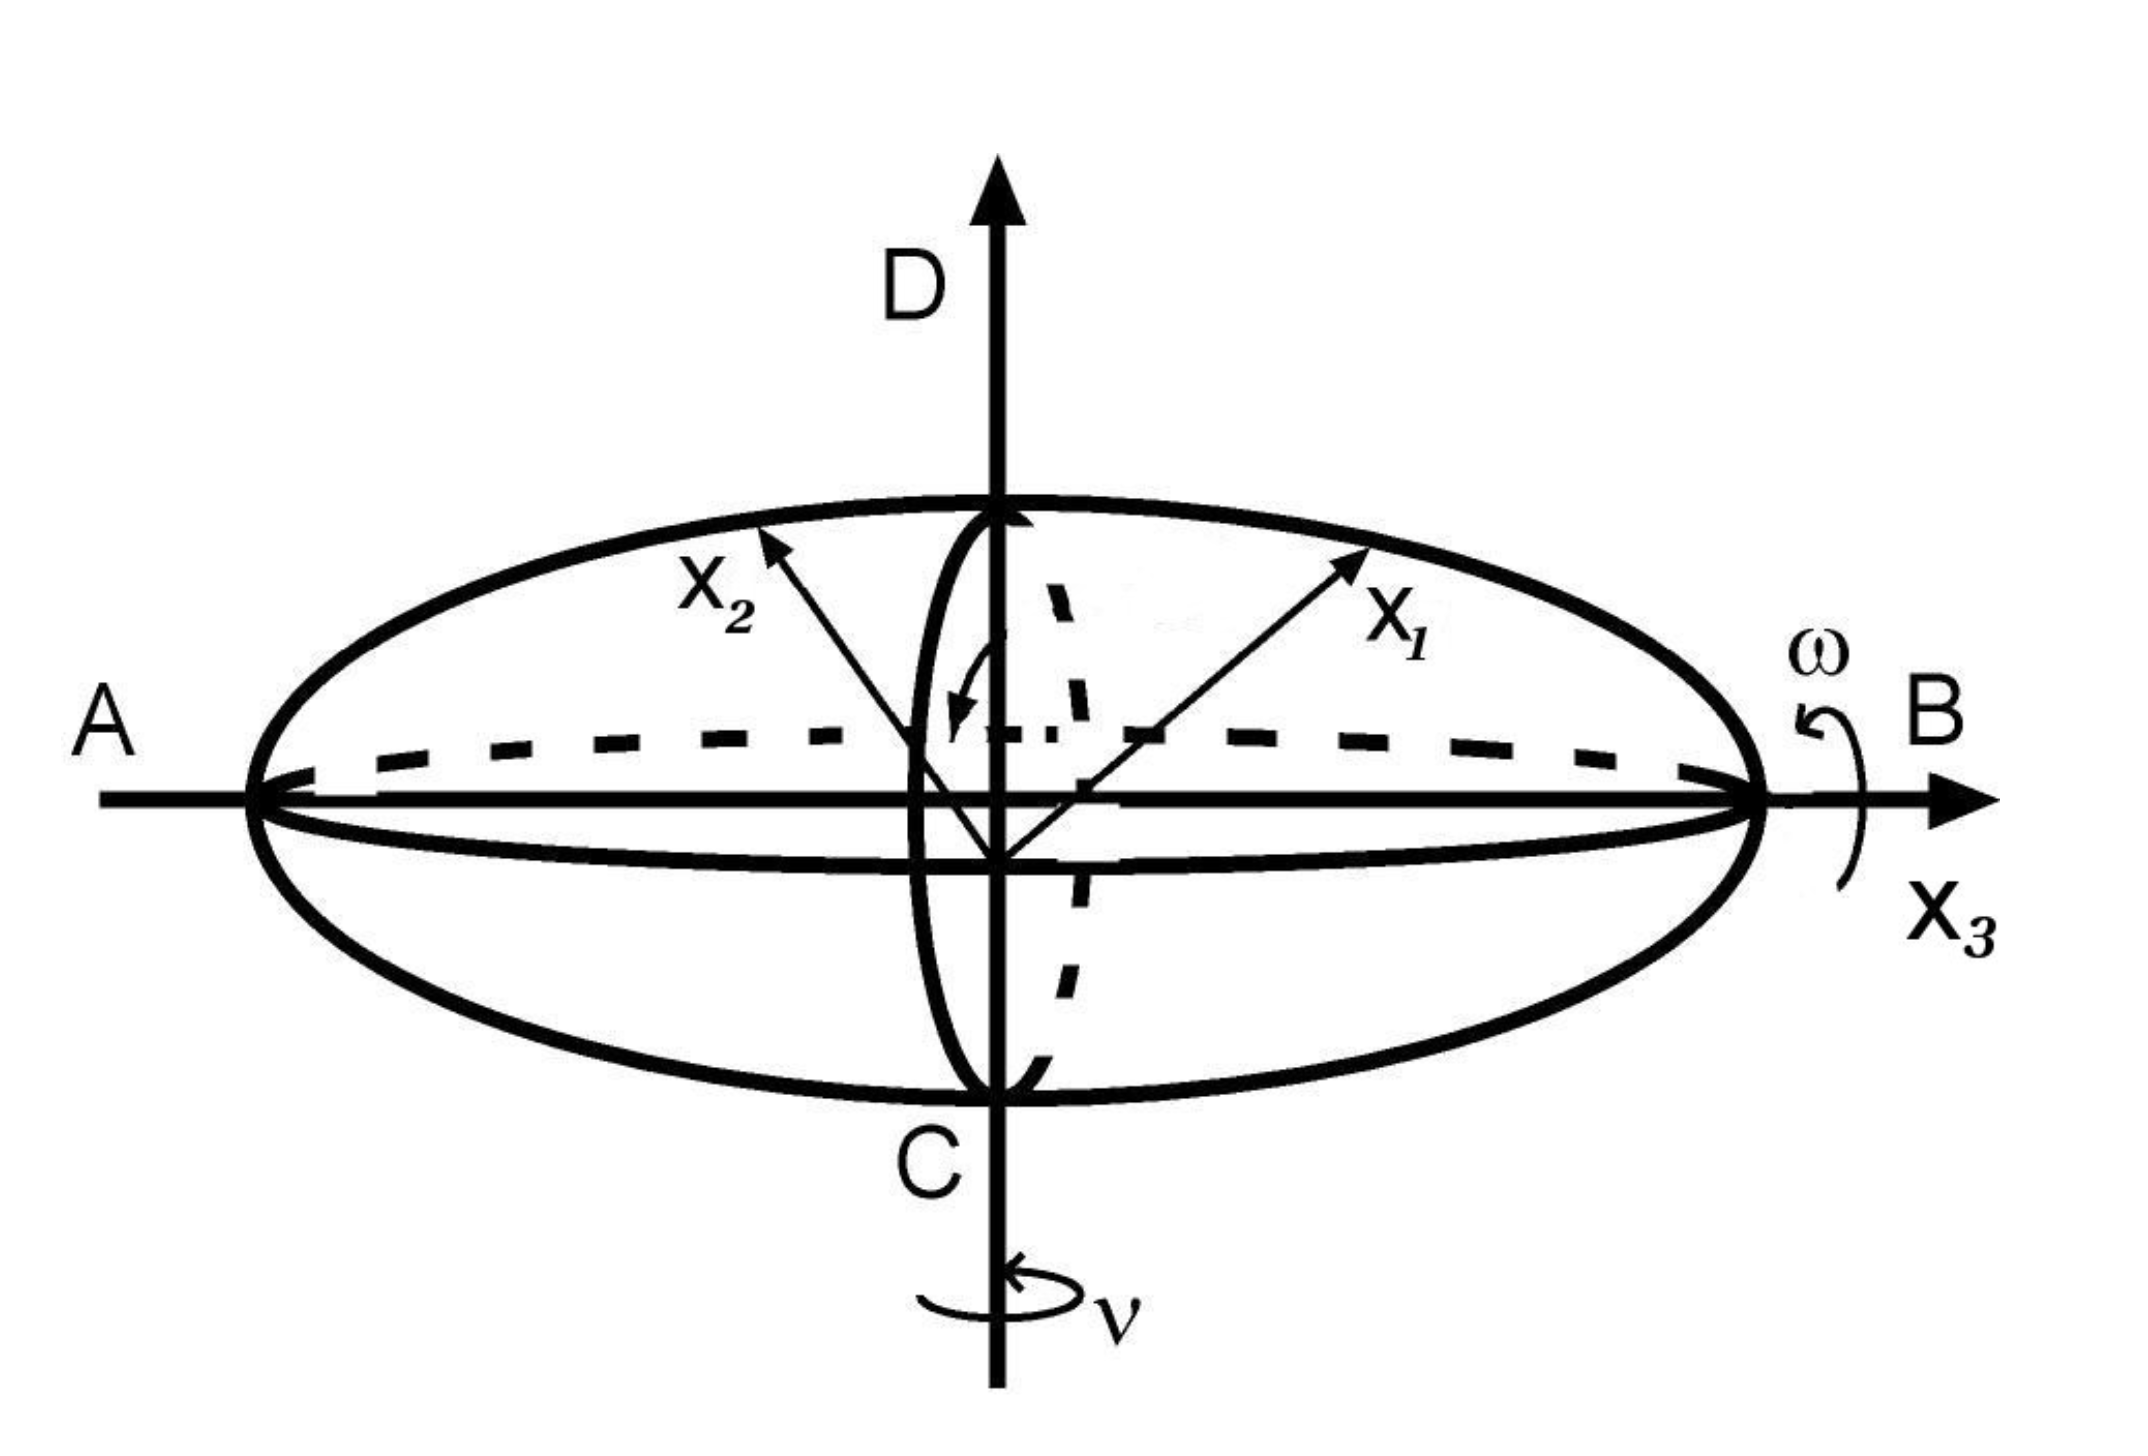
\includegraphics[width=2.0in]{Figuras/Elipsoide.png}
		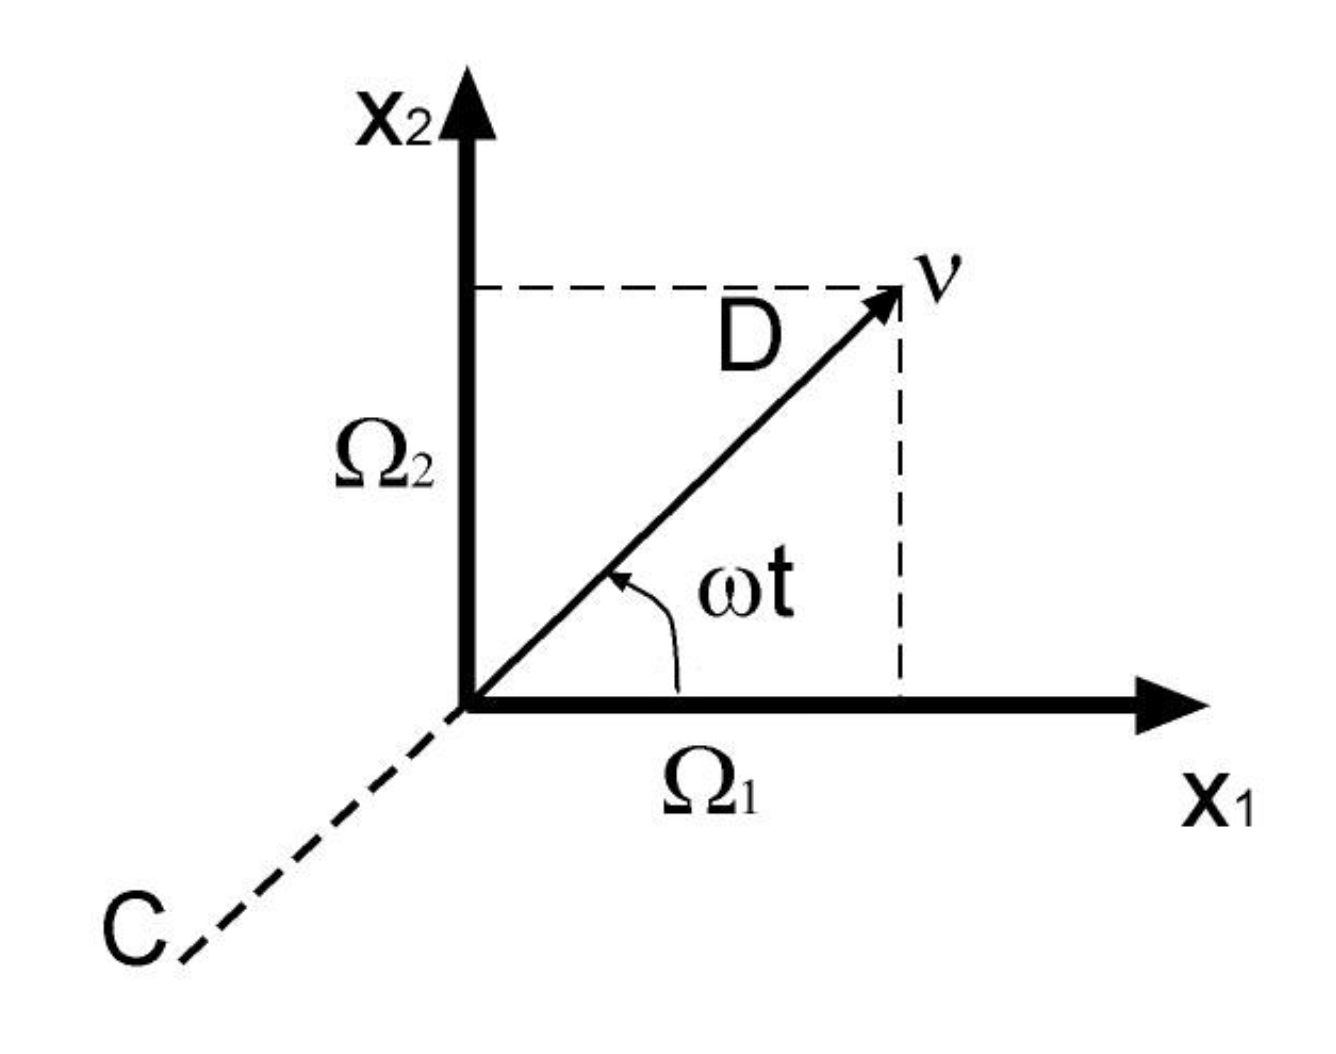
\includegraphics[width=1.5in]{Figuras/PlanosElipsoide.png}
   	\end{figure}
	\item<2-> Escogemos eje $A B$ en la direcci�n $x_3$. Entonces los ejes $x_1$ y $x_2$ rotan alrededor de $A B=x_3$. La direcci�n de $\omega$ es a lo largo de $x_3$ y la direcci�n de $\nu$ est� sobre el plano $\left(x_1, x_2\right)$.
	\item<3-> Las componentes $\boldsymbol{\Omega}=\left(\Omega_1, \Omega_2, \Omega_3\right)$ son
	 $\Omega_1 =\nu \cos \omega t $, $\Omega_2 =\nu \operatorname{sen} \omega t$ y $\Omega_3 =\omega$,
	 \item<4-> Finalmente $T=T_{\text {rot }}  =\frac{1}{2} I_{11} \Omega_1^2+\frac{1}{2} I_{22} \Omega_2^2+\frac{1}{2} I_{33} \Omega_3^2 \Rightarrow$ $ T=\frac{1}{2}\left(I_{11} \cos ^2 \omega t+I_{22} \operatorname{sen} ^2 \omega t\right) \nu^2+\frac{1}{2} I_{33} \omega^2$
\end{itemize}
}
  
\end{document}

	\begin{figure}[t]
		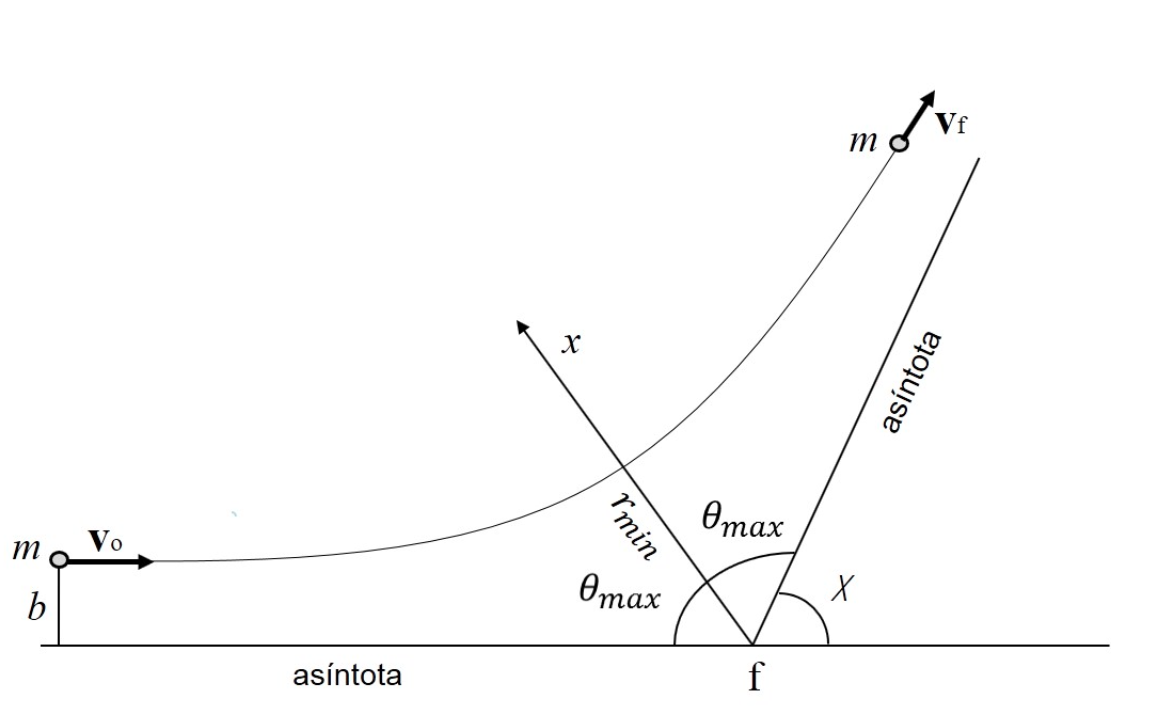
\includegraphics[width=1.8in]{Figuras/Dispersion.png}
   	\end{figure}

%%%%% Diapo 2
\section{Secci�n}
\frame{
\frametitle{T�tulo transparencia}
\begin{itemize}  
	\item<1-> 
\end{itemize}
}
%%%%% Diapo 2
\section{Secci�n}
\frame{
\frametitle{T�tulo transparencia}
\begin{itemize}  
	\item<1-> 
\end{itemize}
}
%%%%% Diapo 2
\section{Secci�n}
\frame{
\frametitle{T�tulo transparencia}
\begin{itemize}  
	\item<1-> 
\end{itemize}
}
%%%%% Diapo Fin
\section{Recapitulando}
\frame{
  \frametitle{Recapitulando}
En presentaci�n consideramos
  \begin{enumerate}
  	\item<1->
   \end{enumerate}
}
	
